\documentclass[a4paper,12pt]{article}
../../../papers/PJTpreamble.tex
\usepackage{chngcntr}

\newenvironment{proof}[1][Proof]{\begin{trivlist}
\item[\hskip \labelsep {\bfseries #1}]}{\end{trivlist}}
%\newenvironment{definition}[1][Definition]{\begin{trivlist}\item[\hskip \labelsep {\bfseries #1}]}{\end{trivlist}}
\newenvironment{example}[1][Example]{\begin{trivlist}
\item[\hskip \labelsep {\bfseries #1}]}{\end{trivlist}}
%\newenvironment{remark}[1][Remark]{\begin{trivlist}\item[\hskip \labelsep {\bfseries #1}]}{\end{trivlist}}

\newcommand{\qed}{\nobreak \ifvmode \relax \else
      \ifdim\lastskip<1.5em \hskip-\lastskip
      \hskip1.5em plus0em minus0.5em \fi \nobreak
      \vrule height0.75em width0.5em depth0.25em\fi}

      \begin{document}
\begin{corollary}
With the assumptions of Theorem \ref{theorem} and affine linear vector fields $F^k$, the initial condition of the iPRC, $z(t)$, must satisfy
 \begin{equation}\label{eq:eigenvalue}
z^1_0=B z^1_0,
\end{equation}
where
\begin{equation}
B=M^{K}e^{A^{K}t_K}\cdots M^1e^{A^1 t_1},
\end{equation}
$t_k$ is the time of flight through the $k^{th}$ region, $e^{A^{k}}$ is the matrix exponential of $A^k = -\left(DF^k\right)^\intercal$.  Eq.~\eqref{eq:eigenvalue} and the normalization condition,
 \begin{equation}\label{eq:normalization}
F_0^1\cdot z^1_0=\frac{1}{T},
\end{equation}
yield a unique solution for the initial condition, $z_0^1 \in \mathbb{R}^2$, provided the nullspace of the matrix $B-I$ does not have dimension greater than one.
\label{corl:circuit}\end{corollary}

%It is straightforward to show that
%\begin{eqnarray}
%\det (M^R) &=& \frac{\hat{n}_R\cdot F^R_f}{\hat{n}_R\cdot F_0^{R+1}}\\
%\text{tr} (M^R)&=&1+\frac{\hat{n}_R\cdot F^R_f}{\hat{n}_R\cdot F_0^{R+1}}\\
%Q(M^R)=\text{tr}(M^R)^2-4\det(M^R) &=& \left( \frac{\hat{n}_R\cdot F^R_f}{\hat{n}_R\cdot F_0^{R+1}}-1 \right)^2
%\end{eqnarray}
%from which it follows that the eigenvalues of $M^R$ are exactly
%\begin{equation}
%\lambda\in\left\{1,\frac{\hat{n}_R\cdot F^R_f}{\hat{n}_R\cdot F_0^{R+1}}\right\}.
%\end{equation}
%Note that $\hat{n}_R\cdot F^R_f$ is the speed at which the limit cycle is traveling
%in the direction normal to the boundary when reaches crossing time $t_R$ from region $R$, and $\hat{n}_R\cdot F_0^{R+1}$ is the speed with which it enters region $R+1$, so the term showing up in the eigenvalues is the ratio of the normal velocity components  approaching and leaving the boundary.

%If, in addition, the flow is piecewise linear, with constant adjoint Jacobian matrices $A^R=-D(F^R)^\trans$, 
%and we define $\Delta_R=t_R-t_{R-1}$ to be the traversal time for region $R$, 
\begin{proof}
Let $z_0^1$ be the initial condition for the adjoint equation, and let $z_i^1(0)$ be the $i^{th}$ component.  To prove the corollary, we solve the adjoint equation for region $R$, apply the matrix $M^R$ at the boundary to calculate jumps in the iPRC, then repeat the process for region $R+1$ and continue inductively for subsequent regions.

Beginning with an arbitrary region, which we label $R=1$, the solution at $t_1$ (the time of flight through region $R=1$), is
\begin{equation}
 z^1_f = e^{A^1t_1}z^1_0,
\end{equation}
where $A(t) = -DF^T(\gamma(t))$ is constant.  The initial condition for the next region, $z_0^2$, is equal to the final value of the previous region with jumps calculated by $M^1$,
\begin{equation}
  z^2_0 = M^1 e^{A^1 t_1}z^1_0.
\end{equation}
We can continue this procedure inductively for the initial condition of the $K^{th}$ iPRC,
\begin{equation}
z^K_0=M^{K-1}e^{A^{K-1}t_{K-1}}\cdots M^1e^{A^1 t_1}z^1_0.
\end{equation}
Since the underlying limit cycle is periodic, $z(t)$ must be periodic, therefore $z^{K+1}(0) = z^1(0)$, and
\begin{equation}
 z^{1}_0=M^{K}e^{A^{K}t^{K}}M^{K-1}e^{A^{K-1}t^{K-1}}\cdots M^1e^{A^1t^1}z^1_0.
\end{equation}
The first statement in the corollary follows upon collapsing the matrix product into a $2\times2$ matrix $B$.

To prove uniqueness, we follow a procedure similar to that used in \cite{Coombes:2008:SIADS} and apply Eqs.~\eqref{eq:eigenvalue} and \eqref{eq:normalization}.  Rewriting Eq.~\eqref{eq:eigenvalue},
\begin{equation}
 \begin{split}
  \matrix{c}{z_1^1(0) \\ z_2^1(0)} &= z_0^1 =  B z_0^1\\
  &= \matrix{c}{b_{11} z_1^1(0) + b_{12}z_2^1(0)\\b_{21} z_1^1(0) + b_{22} z_2^1(0)}.
 \end{split}
\label{eq:Bmatrixfull}\end{equation}

we can rewrite Eq.~\eqref{eq:Bmatrixfull} as a system of equations for $z_1^1(0)$ and $z_2^1(0)$,
\begin{equation}
 \begin{split}
  z_1^1(0)(1-b_{11}) &= b_{12}z_2^1(0),\\
  z_2^1(0)(1-b_{22}) &=b_{21}z_1^1(0).
 \end{split}
\end{equation}

WLOG, we choose the first of Eq.~\eqref{eq:Bmatrixfull} combined with Eq.~\eqref{eq:normalization} to form the system of equations,
\begin{equation}
 \begin{split}
 z_1^1(0) f_0^1 + z_2^1(0)g_0^1 &= \frac{1}{T},\\
  z_1^1(0)(b_{11}-1) + b_{12}z_2^1(0) &=0,
 \end{split}
\end{equation}
which we solve by inverting the matrix in the equivalent equation,
\begin{equation}
\matrix{cc}{f_0^1 & g_0^1\\(b_{11}-1) & b_{12}} \matrix{c}{z_1^1(0)\\z_2^1(0)} = \matrix{c}{\frac{1}{T}\\0},
\end{equation}
which establishes uniqueness of the solution, provided 
\begin{equation}\det \matrix{cc}{f_0^1 & g_0^1\\(b_{11}-1) & b_{12}} \neq 0.\label{eq:uniqueness-of-initial-cond}\end{equation} 
From the periodicity of the solution $z(t)$, we know that $B$ has at least one eigenvector with unit eigenvalue.  The condition (\ref{eq:uniqueness-of-initial-cond}) is equivalent to requiring that the matrix $B-I$ have a null space of not greater than one dimension.
\qed%$\Box$
\end{proof}
% which yields
% \begin{equation}
%  \matrix{c}{z_1^1(0)\\z_2^1(0)} = \matrix{cc}{1/f_0^1 & 0\\\frac{b_{21}}{f_0^1 (1-b_{22})} & 1/(1-b_{22})}  \matrix{c}{\frac{1}{T} - \frac{1-b_{11}}{b_{12}} g_0^1\\0},
% \end{equation}



%As a condition for this equation to be solvable, the matrix $B$ has to have at least one unit eigenvalue.  In addition, we have not yet used the normalization condition

%where $T=\sum_{k=1}^N \Delta_k$ is the total period, or the sum of the transit times through all $N$ regions.  
%These two conditions (\ref{eq:eigenvalue} and \ref{eq:normalization}) should (we hope?) lead to a unique solution for $z^1_0$, and hence $z(t)$.  
\subsection{Applications}
\subsubsection{Piecewise Linear Morris-Lecar}
The Morris-Lecar model is a conductance-based planar neurobiological model developed to understand oscillations in barnacle muscle fiber \cite{MorrisLecar:1981} (see Appendix \ref{app:morris-lecar}).  In \cite{Coombes:2008:SIADS}, Coombes constructed a piecewise linear approximation to the Morris-Lecar model for use in gap junction coupled networks (see Appendix \ref{app:pml}).  Following the notation used in \cite{Coombes:2008:SIADS}, since each region follows piecewise linear dynamics, we can solve for the iPRC, $Q_\mu(t) \in \mathbb{R}^2$, of region number $\mu$.  Coombes provides an ad-hoc derivation of the iPRC, implicitly taking the matrix $M^R$ to be the identity for each boundary crossing.  Here we apply Theorem \ref{theorem} and prove that $M^R$ is indeed the identity for all boundaries.

By Theorem \ref{theorem}, discontinuities over the boundary satisfy
\begin{equation}
Q_{\mu+1}(0) = \left. M^{R} \right |_{R=\mu}   Q_\mu(T_\mu),
\end{equation}
where $T_\mu$ is the time it takes the limit cycle solution to traverse region $\mu$.  We will calculate the matrix $M^R$ at each boundary.  To avoid possible confusion with the matrix exponent, we define $M_R := M^R$.

First, consider the boundary between regions $4$ and $1$.  By Theorem \ref{theorem},
\begin{equation}
 Q_1(0) = M_4Q_4(T_4).
\end{equation}
By definition, the components $f^4$ and $f^1$ are equivalent at this boundary, so assign a constant to represent both values, $A := f_f^4 = f_0^1$.  Then
\begin{equation}
 \begin{split}
   M_4 = \matrix{cc}{A & g_0^{1}\\0 & 1}^{-1} \matrix{cc}{A & g_f^{4}\\0 & 1}  &= \frac{1}{A}\matrix{cc}{1 & -g_0^{1}\\0 & A} \matrix{cc}{A & g_f^{4}\\0 & 1}\\
   &=\matrix{cc}{1 & (g_f^4-g_0^1)/A\\0 & 1}.\\
 \end{split}
\end{equation}
By definition, 
\begin{equation}
\begin{split}
g_f^{4} &=(b - \gamma_1 w^* + b^* \gamma_1 -b)/\gamma_1,\\
  g_0^1 &= (b - \gamma_2 w^* + b^* \gamma_2 -b)/\gamma_2,
\end{split}
\end{equation}
so the difference is zero,
\begin{equation}
 \matrix{cc}{1 & (g_f^4-g_0^1)/A\\0 & 1} = \matrix{cc}{1 & 0\\0 & 1}.
\end{equation}
Thus the vector field at which the limit cycle crosses the boundary agrees on both sides, and
\begin{equation}
 Q_4(T_4) =  Q_1(0),
\end{equation}
so there is no discontinuity in the iPRC across the boundary between regions 4 and 1.  Calculations for the transition from region 4 to region 3 result in the identity matrix, because again, the vector field in region 3 agrees with the vector field in region 1 at the point at which the limit cycle crosses the boundary.

Next, consider the boundary between regions 1 and 2.  In this transition, the definition of the first component of the vector field changes from $f_f^1$ to $f_0^2$, but the second component of the vector field does not (by construction).  Let the constant $A$ represent both values, $A:=g_f^1=g_0^2$.  The matrix $M_1 := M^1$ is then
\begin{equation}
\begin{split}
 M_1 = \matrix{cc}{f_0^2 & A\\0 & 1}^{-1} \matrix{cc}{f_f^2 & A\\0 & 1}  &= \frac{1}{f_0^2}\matrix{cc}{1 & -A\\0 & f_0^2}\matrix{cc}{f_f^2 & A\\0 & 1}\\
   &= \frac{1}{f_0^2}\matrix{cc}{f_f^1 & 0\\0 & f_0^2}\\
   &= \matrix{cc}{f_f^1/f_0^2 & 0\\0 & 1}.
   \end{split}
\end{equation}
By definition,
\begin{equation}
\begin{split}
  f_f^1/f_0^2 &= \frac{v_{th}^1 - a - w^* + I}{1-v_{th}^1 - w^* + I}\\
  &= \frac{(1+a)/2 - a - w^* + I}{1- (1+a)/2- w^* + I}\\
  &= 1.
\end{split}
\end{equation}
Therefore the vector fields agree on both sides at the point at which the limit cycle crosses, and
\begin{equation}
 Q_1(T_1) =  Q_2(0),
\end{equation}
so there is no discontinuity in the iPRC across the boundary between regions 1 and 2.  Once again, the vector field along the limit cycle from region 2 to region 3 agree on both sides, so $M^R$ evaluates to the identity matrix for the boundary between regions 2 and 3.

\begin{figure}[h!]
\begin{center} 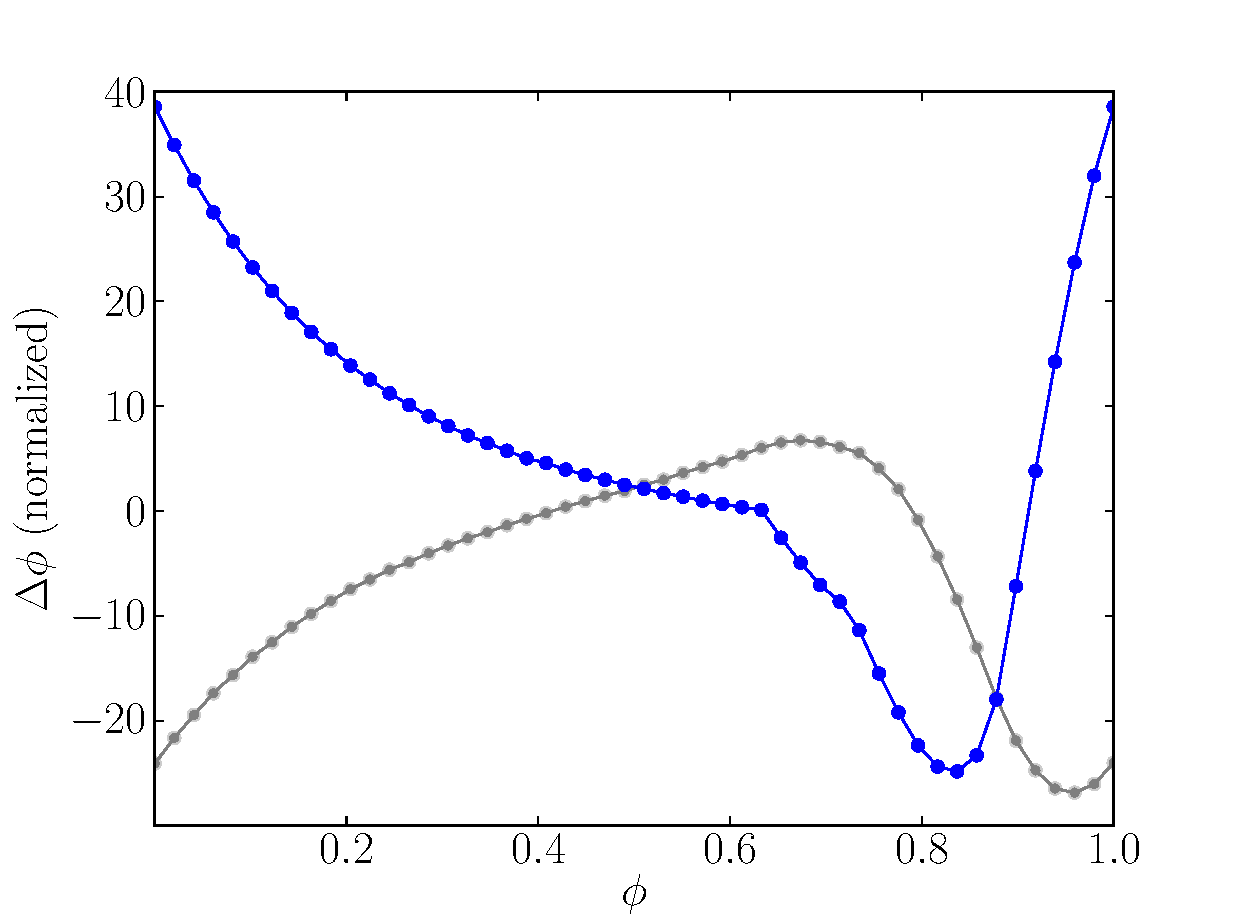
\includegraphics[width=1\textwidth]{pml_prc_fig.pdf}\end{center}
\caption[Numerical iPRCs of the PML system]{Numerical iPRCs of the PML system. Blue: perturbations in the positive horizontal direction. Gray: perturbations in the positive vertical direction.  There are no discontinuities in either iPRC. Copyright~\copyright~~2008 Society for Industrial and Applied Mathematics.  Reprinted with permission.  All rights reserved.}
\label{fig:pml_iprc}\end{figure}

 This completes the proof that the iPRC of both coordinates in the PML model is continuous across all boundaries (though not necessarily $C^1$).  See Fig.~\ref{fig:pml_iprc} for the numerical iPRC that confirms this result.

\subsubsection{McKean Model}
The McKean model was developed as a piecewise linear approximation to the FitzHugh-Nagumo model \cite{McKean1970}.  Let the McKean model be defined as in Appendix \ref{app:mckean}.  We use similar methods as in the previous section.  By definition, the second coordinate of the vector field is the same for all regions, so we define $A_R = g_0^R = g_f^R$ for each region $R$.  We begin with the boundary between regions 4 and 1, derive the matrix $M_R:=M^R$, and repeat for the remaining boundaries.

In the transition between regions 4 and 1, we have the matrix
\begin{equation}
\begin{split}
 M_4 &= \matrix{cc}{f_0^1 & A_4\\0 & 1}^{-1} \matrix{cc}{f_f^4 & A_4\\0 & 1}\\
 &=\matrix{cc}{f_f^4/f_0^1 & 0\\0 & 1}.
\end{split}
\end{equation}

By definition,
\begin{equation}
\begin{split}
 f_f^4/f_0^1 &= \frac{-v_{th}^1 - w^* + I}{v_{th}^1-a-w^*+I}\\
 &= \frac{-a/2 - w^* + I}{a/2-a-w^*+I} = 1,
\end{split}
\end{equation}

so $M_1$ is the identity matrix and
\begin{equation}
 Q_1(0) = Q_4(T_4).
\end{equation}

In the transition between regions 1 and 2, $M_1$ is
\begin{equation}
 \begin{split}
  M_1 &= \matrix{cc}{f_0^2 & A_1\\0 & 1}^{-1} \matrix{cc}{f_f^1 & A_1\\0 & 1}\\
  &= \matrix{cc}{f_f^1/f_0^2 & 0\\0 & 1}.
 \end{split}
\end{equation}
Again by definition,
\begin{equation}
 \begin{split}
  f_1^f/f_0^2 = &= \frac{v_{th}^2 - a - w^* + I}{1-v_{th}^2-w^*+I}\\
 &= \frac{1/2-a/2 - w^* + I}{1-(1/2+a/2)-w^*+I} = 1.
 \end{split}
\end{equation}
Therefore $M_2$ is the identity matrix and
\begin{equation}
 Q_2(0) = Q_1(T_1).
\end{equation}

The transition between region 2 and region 3 and and the transition between region 3 and region 4, we have the matrices
\begin{equation}
 \begin{split}
  M_2 &= \matrix{cc}{f_f^2/f_0^3 & 0\\0 & 1},\\
  M_3 &= \matrix{cc}{f_f^3/f_0^4 & 0\\0 & 1},
 \end{split}
\end{equation}
which each evaluate to the identity by the calculations above.

\begin{figure}[h!]
\begin{center} 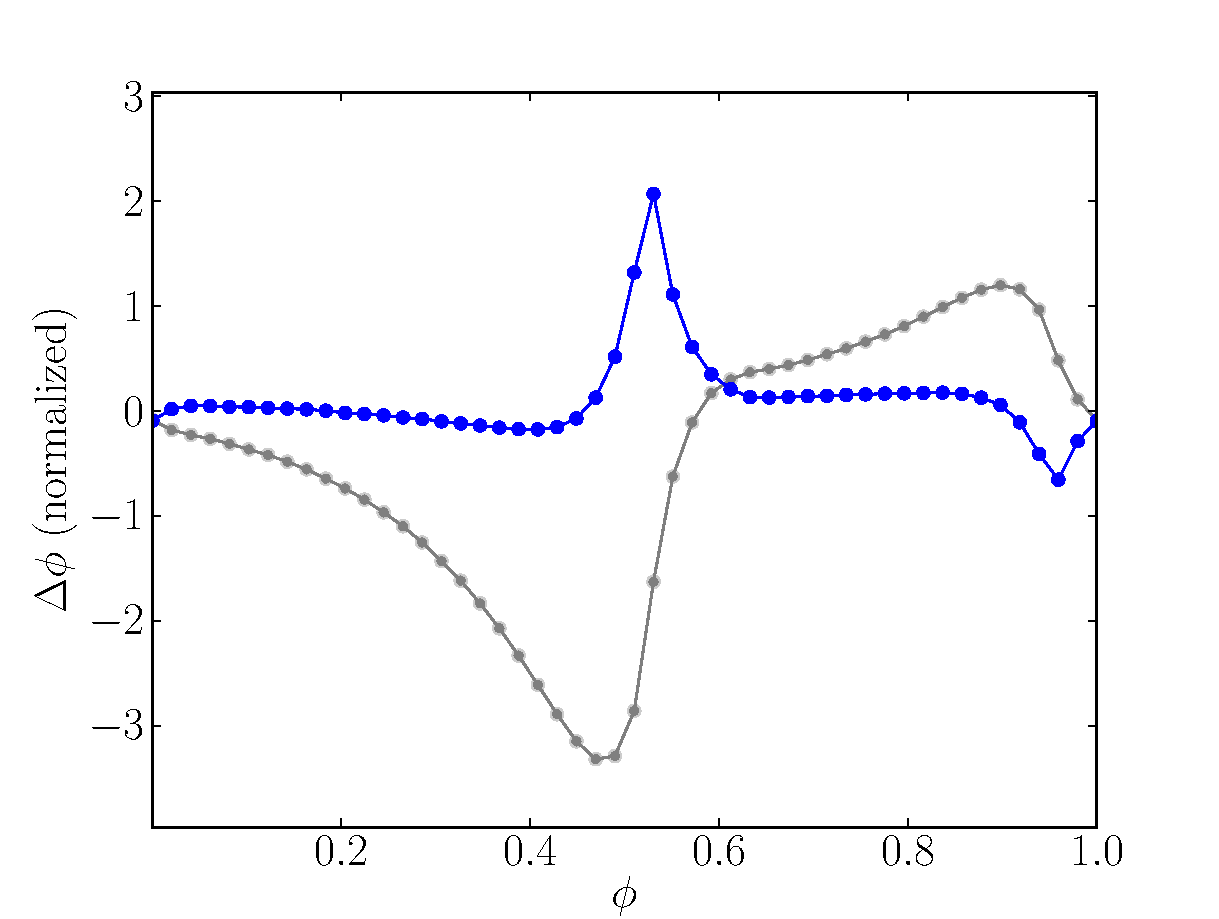
\includegraphics[width=1\textwidth]{pmk_prc_fig.pdf}\end{center}
\caption[Numerical iPRCs of the McKean model]{Numerical iPRCs of the McKean model. Blue: perturbations in the positive horizontal direction. Gray: perturbations in the positive vertical direction.  There are no discontinuities in either iPRC. Copyright~\copyright ~2008 Society for Industrial and Applied Mathematics.  Reprinted with permission.  All rights reserved.}
\label{fig:pmk_iprc}\end{figure}

Again, the iPRCs of both coordinates are continuous (but not necessarily $C^1$).  See Fig.~\ref{fig:pmk_iprc} for the numerical iPRC that confirms this result.  We direct the reader to \cite{Coombes:2008:SIADS} for explicit expressions for the iPRC of both systems.

\subsubsection{Iris System}
The iris system is a piecewise linear dynamical system developed by Shaw et al to approximate the smooth sine system, which exhibits a heteroclinic cycle and a family of one-parameter limit cycles \cite{ShawParkChielThomas2012SIADS}.  When the bifurcation parameter, $a$, is small and positive, there exists a limit cycle, with transit time $T = \log(1/u)$ for entry coordinate $u$. We further define the phase $\theta = t/T$ for one region.  Let the iris system be as defined in Appendix \ref{app:iris}.  For the Southwest (SW) square of the iris system, we directly can solve for the iPRC, $Z$, using basic methods in differential equations.  The solutions are,
\begin{equation}
\begin{split}
 Z_1(\theta) &= Z_1(0) e^{\lambda \theta T},\\
 Z_2(\theta) &= Z_2(0) e^{-\theta T},
\end{split}
\label{eq:zi}\end{equation}
We exploit the symmetry of the iris system to efficiently obtain an exact solution, which we then compare to the solution for the adjoint equation from Shaw et al.  Recall Eq.~\eqref{eq:normalization},
\begin{equation}
 F_0^1 \cdot z_0^1 = 1/T.
\end{equation}
For the iris system, $F_0 = (-\lambda, u)$, so in order for the initial conditions of the iPRC to satisfy Eq.~\eqref{eq:normalization}, we have that
\begin{equation}
\begin{split}
 Z_1(0) &= \frac{c}{\lambda},\\
 Z_2(0) &= \frac{(1/T+c)}{u},
 \end{split}
\label{eq:z0}\end{equation}
where $u$ is the entry coordinate of the SW iris square.  We show below that one can solve for the constant $c$, which turns out to be
\begin{equation}
 c = \frac{1}{T}\frac{\kappa}{u-\kappa},
\label{eq:c}\end{equation}
where $\kappa = \lambda u^{\lambda}$ and $u$ is again the entry coordinate. The derivation of these equations follows.
% \begin{figure}[h!]
% \begin{center}
% \includegraphics[width=1\textwidth]{adjoint_iprc.png}
% \caption[Comparison between adjoint iPRC and analytical iPRC]{Comparison between adjoint iPRC and analytical iPRC.  The adjoint iPRC closely resembles that of the original analytic iPRC.}\label{adjoint_iprc}
% \end{center}
% \end{figure}

First we show how to solve for the iris iPRC in terms of phase, with initial conditions left unknown.  We begin with the adjoint equation,
\begin{equation}
 \frac{dz}{dt} = -A(t)^T z.
\end{equation}
We want to solve the adjoint equation in terms of phase $\phi \in [0,1)$.  Note that since $t = \phi T$ and $d t = T d \phi$,  The Jacobian of the nondimensionalized iris system in the bottom left corner,
\begin{align}
 \frac{1}{T}\frac{ds(\phi)}{d\phi} &= -\lambda s(\phi)\\
 \frac{1}{T}\frac{du(\phi)}{d\phi} &= u(\phi),
\end{align}
is a constant matrix:
\begin{equation}
 J_{SW}(\phi) = T \left( \begin{array}{cc} -\lambda & 0 \\ 0 & 1 \end{array} \right ),
\end{equation}
where $J_{SW}$ denotes the Jacobian in the SW square.  Since $J_{SW}$ is Hermitian, we can use this matrix (multiplied by $-1$) to solve the adjoint equation.  This requires solving for the system of equations
\begin{align}
\left ( \begin{array}{c} \frac{dZ_1}{d\phi}\\ \frac{dZ_2}{d\phi} \end{array} \right )  &= T J_{LL} \left ( \begin{array}{c} Z_1 \\ Z_2 \end{array} \right)\\
&= T \left (\begin{array}{c}
    \lambda Z_1 \\ -Z_2
   \end{array} \right ),
\end{align}
which yields the solutions in terms of phase,
\begin{align}
 Z_1(\theta) & = Z_1(0) e^{\lambda \theta T},\\
 Z_2(\theta) & = Z_2(0) e^{-\theta T},
\end{align}
where $\theta \in [0,1)$, and $T$ is the time of flight within a particular square.  The functions $Z_1$, $Z_2$ represent the iPRC for perturbations in the $x$- and $y$- coordinates, respectively (restricted to the SW square).
% We can solve for the initial condition of each equation by solving for the normalization condition
% \begin{equation}
% \left \langle Z(\phi),T \frac{dX_\gamma(\phi)}{d\phi} \right \rangle= \left \langle Z(\phi),T J_{LL}(\phi) \right \rangle =  1,
% \end{equation}
% where $X_\gamma$ represents the limit cycle trajectory. By linearity, we can solve the equivalent expression,
% \begin{equation}
% \left \langle Z(\phi),J_{LL}(\phi) \right \rangle= \frac{1}{T}.
% \end{equation}
% In particular, the equation must hold true for $\phi = t = 0$.  The term $J_{LL}(0)$ is the Jacobian matrix multiplied against the column vector of the initial entry position, $(1,u)^T$.  So at $\phi = t = 0$, we have
% \begin{equation}
% \begin{split}
%  \left \langle (Z_1(0), Z_2(0))^T, (-\lambda, u)^T \right \rangle &= 1/T\\
%  -\lambda Z_1(0) + Z_2(0) u &= 1/T.
%  \end{split}
% \end{equation}
% 
Recall that in order for the initial conditions of the iPRC of the iris system to satisfy Eq.~\eqref{eq:normalization}, the initial conditions take the form
\begin{align}
 Z_1(0) &= \frac{c}{\lambda},\\
 Z_2(0) &= \frac{c+1/T}{u}.
\end{align}
We will solve for the constant $c$.  Before we continue, note that the equation for the global iPRC is defined piecewise, and that the global iPRC for perturbations in the positive $s$-direction (in the SW square) becomes perturbations in the positive $u$ direction (NW square).  Moreover, the matrix for Theorem 1 at the boundary between the SW and NW squares (regions 1 and 2) is
\begin{equation}
 M^1 = \matrix{cc}{1 & 0\\
\frac{f^1+f_0^2}{g_0^2} & \frac{g_f^1}{g_0^2}}.
\end{equation}
Therefore, the first component of the iPRC in each square is continuous, and by the symmetry argument above, we must solve
\begin{equation}
\begin{split}
 Z_1(1) &= Z_2(0).
 \end{split}
\end{equation}

Since $\lambda u^\lambda \neq u$,
\begin{equation}
\begin{split}
 Z_1(1) &= Z_2(0)\\
Z_1(0)u^{-\lambda} &= Z_2(0)\\
  \frac{c u^{-\lambda}}{\lambda}  &= \frac{c+1/T}{u}\\
 % \frac{c u^{-\lambda}}{\lambda}  = \frac{c}{u} + \frac{1}{Tu}\\
 %c \left (\frac{u^{-\lambda}}{\lambda}  -  \frac{1}{u}\right )  = \frac{1}{Tu}\\
 c  &= \frac{1}{Tu}  \left (\frac{u^{-\lambda}}{\lambda}  -  \frac{1}{u}\right )^{-1}\\
 %c  = \frac{1}{Tu}  \left (\frac{u^{1-\lambda} - \lambda}{\lambda u}\right )^{-1}\\
 %c  = \frac{1}{T}  \left (\frac{\lambda}{u^{1-\lambda} - \lambda}\right )\\
 c  &= \frac{1}{T}  \left (\frac{\lambda u^\lambda}{u - \lambda u^\lambda}\right ).\\
 \end{split}
\end{equation}
When $c$ is substituted back into $Z_1(0)$, this yields the full iPRC derived by the adjoint equation for the SW square and perturbations in the horizontal direction,
\begin{equation}
Z_1(\phi) = \frac{1}{T}  \left (\frac{u^\lambda}{u - \lambda u^\lambda}\right ) e^{\lambda \phi T}.
\end{equation}
We can simplify into the equivalent expression,
\begin{equation}
Z_1(\phi) = \frac{1}{T}  \left (\frac{u^\lambda}{u- \lambda u^\lambda}\right ) u^{-\lambda \phi}.
\end{equation}
The direct iPRC from Shaw et al (2012), for the SW square and perturbations in the horizontal direction is
\begin{equation}
Z_x(\phi) = \frac{u^{\lambda(1-\phi)}}{T(u-\lambda u^\lambda)}.
\end{equation}
Equivalence is clear.

We now derive $Z_2(\theta)$ using the same $c$.  First combine Eqs.~\eqref{eq:z0} and ~\eqref{eq:c} and expose $\kappa$, which yields the expression
\begin{equation}
\begin{split}
  Z_2(0) &= \frac{1+\left( \frac{1}{T}\frac{\kappa}{u-\kappa} \right ) T}{T u}\\
  &=\frac{(u-\kappa)+\kappa}{T u (u-\kappa)}\\
  &=\frac{1}{T (u-\lambda u^\lambda)}.
\end{split}
\end{equation}
combining this with Eq.~\eqref{eq:zi} yields the exact formula for the iPRC in the second coordinate,
\begin{equation}
\begin{split}
 Z_2(\theta) &= \frac{e^{-\theta T}}{T (u-\lambda u^\lambda)}\\
 &=\frac{u^{\theta}}{T (u-\lambda u^\lambda)}.
\end{split}
\end{equation}
The direct iPRC from Shaw et al (2012), for the SW square and perturbations in the vertical direction is
\begin{equation}
Z_y(\phi) = \frac{u^{\phi}}{T(u-\lambda u^\lambda)}.
\end{equation}
Again, equivalence is clear.
\end{document}